\documentclass[english,,man]{apa6}
\usepackage{lmodern}
\usepackage{amssymb,amsmath}
\usepackage{ifxetex,ifluatex}
\usepackage{fixltx2e} % provides \textsubscript
\ifnum 0\ifxetex 1\fi\ifluatex 1\fi=0 % if pdftex
  \usepackage[T1]{fontenc}
  \usepackage[utf8]{inputenc}
\else % if luatex or xelatex
  \ifxetex
    \usepackage{mathspec}
  \else
    \usepackage{fontspec}
  \fi
  \defaultfontfeatures{Ligatures=TeX,Scale=MatchLowercase}
\fi
% use upquote if available, for straight quotes in verbatim environments
\IfFileExists{upquote.sty}{\usepackage{upquote}}{}
% use microtype if available
\IfFileExists{microtype.sty}{%
\usepackage{microtype}
\UseMicrotypeSet[protrusion]{basicmath} % disable protrusion for tt fonts
}{}
\usepackage{hyperref}
\hypersetup{unicode=true,
            pdftitle={Process Principles},
            pdfauthor={\ldots{}},
            pdfkeywords={\ldots{}.},
            pdfborder={0 0 0},
            breaklinks=true}
\urlstyle{same}  % don't use monospace font for urls
\ifnum 0\ifxetex 1\fi\ifluatex 1\fi=0 % if pdftex
  \usepackage[shorthands=off,main=english]{babel}
\else
  \usepackage{polyglossia}
  \setmainlanguage[]{english}
\fi
\usepackage{graphicx,grffile}
\makeatletter
\def\maxwidth{\ifdim\Gin@nat@width>\linewidth\linewidth\else\Gin@nat@width\fi}
\def\maxheight{\ifdim\Gin@nat@height>\textheight\textheight\else\Gin@nat@height\fi}
\makeatother
% Scale images if necessary, so that they will not overflow the page
% margins by default, and it is still possible to overwrite the defaults
% using explicit options in \includegraphics[width, height, ...]{}
\setkeys{Gin}{width=\maxwidth,height=\maxheight,keepaspectratio}
\IfFileExists{parskip.sty}{%
\usepackage{parskip}
}{% else
\setlength{\parindent}{0pt}
\setlength{\parskip}{6pt plus 2pt minus 1pt}
}
\setlength{\emergencystretch}{3em}  % prevent overfull lines
\providecommand{\tightlist}{%
  \setlength{\itemsep}{0pt}\setlength{\parskip}{0pt}}
\setcounter{secnumdepth}{0}
% Redefines (sub)paragraphs to behave more like sections
\ifx\paragraph\undefined\else
\let\oldparagraph\paragraph
\renewcommand{\paragraph}[1]{\oldparagraph{#1}\mbox{}}
\fi
\ifx\subparagraph\undefined\else
\let\oldsubparagraph\subparagraph
\renewcommand{\subparagraph}[1]{\oldsubparagraph{#1}\mbox{}}
\fi

%%% Use protect on footnotes to avoid problems with footnotes in titles
\let\rmarkdownfootnote\footnote%
\def\footnote{\protect\rmarkdownfootnote}


  \title{Process Principles}
    \author{\ldots{}\textsuperscript{1}}
    \date{}
  
\shorttitle{PROCESS PRINCIPLES}
\affiliation{
\vspace{0.5cm}
\textsuperscript{1} ...}
\keywords{....\newline\indent Word count: 95}
\usepackage{csquotes}
\usepackage{upgreek}
\captionsetup{font=singlespacing,justification=justified}

\usepackage{longtable}
\usepackage{lscape}
\usepackage{multirow}
\usepackage{tabularx}
\usepackage[flushleft]{threeparttable}
\usepackage{threeparttablex}

\newenvironment{lltable}{\begin{landscape}\begin{center}\begin{ThreePartTable}}{\end{ThreePartTable}\end{center}\end{landscape}}

\makeatletter
\newcommand\LastLTentrywidth{1em}
\newlength\longtablewidth
\setlength{\longtablewidth}{1in}
\newcommand{\getlongtablewidth}{\begingroup \ifcsname LT@\roman{LT@tables}\endcsname \global\longtablewidth=0pt \renewcommand{\LT@entry}[2]{\global\advance\longtablewidth by ##2\relax\gdef\LastLTentrywidth{##2}}\@nameuse{LT@\roman{LT@tables}} \fi \endgroup}


\DeclareDelayedFloatFlavor{ThreePartTable}{table}
\DeclareDelayedFloatFlavor{lltable}{table}
\DeclareDelayedFloatFlavor*{longtable}{table}
\makeatletter
\renewcommand{\efloat@iwrite}[1]{\immediate\expandafter\protected@write\csname efloat@post#1\endcsname{}}
\makeatother
\usepackage{lineno}

\linenumbers

\authornote{\ldots{}.

Correspondence concerning this article should be addressed to \ldots{},
\ldots{}. E-mail: \ldots{}}

\abstract{
Begin here\ldots{}


}

\usepackage{amsthm}
\newtheorem{theorem}{Theorem}[section]
\newtheorem{lemma}{Lemma}[section]
\theoremstyle{definition}
\newtheorem{definition}{Definition}[section]
\newtheorem{corollary}{Corollary}[section]
\newtheorem{proposition}{Proposition}[section]
\theoremstyle{definition}
\newtheorem{example}{Example}[section]
\theoremstyle{definition}
\newtheorem{exercise}{Exercise}[section]
\theoremstyle{remark}
\newtheorem*{remark}{Remark}
\newtheorem*{solution}{Solution}
\begin{document}
\maketitle

sys theory math

comp models in computer I could just put these things into the computer.
direct code like a difference equation. but there are other properties
that become apparent when you do so. here they are.

We -- organizational psychologists -- are increasingly interested in
process and dynamic phenomena. Longitudinal studies are becoming more
prevalent in our literature and the number of time points they employ
appears to be growing ({\textbf{???}}). The empirical literature uses
the term \enquote{dynamics} at an expoentially larger rates in recent
years ({\textbf{???}}). A majority of published methods literature now
focuses on longitudinal data analysis ({\textbf{???}}), and there are
now many great reviews on the conceptual and methodological issues
related to process and dynamics ({\textbf{???}}; {\textbf{???}};
{\textbf{???}}; {\textbf{???}}). Moreover, this interest covers many
content areas, including emotional labor ({\textbf{???}};
{\textbf{???}}; {\textbf{???}}), workplace stress and well-being
({\textbf{???}}; {\textbf{???}}), organizatiional performance
({\textbf{???}}), self-regulation ({\textbf{???}}), newcomer adjustment
({\textbf{???}}), justice and trust ({\textbf{???}}), leadership
({\textbf{???}}; {\textbf{???}}; {\textbf{???}}), decision-making
({\textbf{???}}), team performance ({\textbf{???}}), counterproductive
work behaviors ({\textbf{???}}), work-family conflict ({\textbf{???}}),
job satisfaction ({\textbf{???}}), and team emergent states
({\textbf{???}}). In summary, explaining how a process functions appears
to be of great interest to current organizational science.

There are many ways to do so -- alternative representations that we
might use when we want to describe sequences of events and their
relationships. Just as different statistical models can be used to draw
the same inference given the appropriate assumptions about the data
generating process, we can use different forms of explanation to
describe process. For example, Bandura ({\textbf{???}}) and Kuwabara et
al. ({\textbf{???}}), respectively, explain self regulation and lay
beliefs about networking with verbal theories, ({\textbf{???}}) presents
a mathematical explanation of social impressions, and ({\textbf{???}})
employ both mathematical and computational approaches to explain
self-regulation. People use different labels for these strategies -- for
example, qualitative versus quantitative ({\textbf{???}}) or
computational, mathematical, and verbal ({\textbf{???}}) -- but the
point is that researchers describe process in various ways. Moreover,
each approach uses its own terms and principles to represent the
phenomenon.

In this paper, we point out these principles and discuss the different
ways researchers explain process. Our discussion will move across
literature that uses verbal, mathematical, and computational
explanations. These are all ways to represent relationships over time at
different levels of abstraction. For example, we could use a difference
equation to explain the trajctory of one variable over time, or we could
use terms like autoregression, cycles, or periodicity that describe the
same emergent behavior but in a different way. Don't necessarily need to
be causal; we can explain something and it can be causal or non causal.

We provide several contributions in doing so. First, we believe our
discussion will help researchers augment their current approach to
explaining process. It can be helpful to be exposed to different
approaches, provide ideas etc., and we hope our paper provides new ideas
to seasoned researchers in this area. Second, some of the principles are
technical and sophisticated and may not transfer well to researchers
with graduate-level training. The literature on the principles is
technical and hard to follow. Much of this work is not easily accessible
to researchers with the usual methodological and statistical background
obtained from doctoral level training in managemenet; we want to help
distill it. Finally, we discuss ways to study process for researchers
who may not want to want to develop sophisticated math or computational
models. Some people claim that math is the only option. For example,
Pearl (2009) states that any explanation \enquote{worthy of the title
theory must be able to represent causal questions in some mathematical
language} (p.~102). There is also some pressure to produce computational
theories. For example, VANCOUVER COMP MODELS ARE BETTER; AND KOZLOWSKI
COMP FRAMEWORKS ARE BETTER. But there are not many comp modelers in
organizational psychology VANCOUVER ORM; and the social sciences do not
emphasize mathematics as much as some of the more physical sciences
(vancouver point out cites). Moreoever, Renee Thom points out that
sometimes qualitative representations produce more error than their
quantitative counterparts but nonetheless are better clues to the
underlying process. We do not claim that one approach is better or worse
than another; we simply want to describe process principles from
different domains to give researchers alternative ways of talking about,
specifying, and representing process behavior.

Below, we do these things. There are other excellent papers on aspects
that we will not cover. Ployhart and Vandenberg discuss how to design
and analyze a longitudinal study, Pitariu and Ployhart how to propose
dynamic hypotheses, and Wang provides an overview of dynamic statistical
models. In this paper, conversely, we focus solely on principles
researchers use when they explain process.

\hypertarget{what-is-process}{%
\section{What is process}\label{what-is-process}}

\hypertarget{dymamics}{%
\subsection{Dymamics}\label{dymamics}}

The system has memory. The past has memory. Monge: \enquote{In most
forms of dynamic analysis it is essential to know how variables depend
unpon their own past history} p.~409 Wang: \enquote{A dynamic model can
be defined as a representation of a system that evolves over time. In
particular it describes how the system evolves from a given state at
time \emph{t} to another state at time \emph{t + 1} as goverened by the
transition rules and potential external inputs.} p.~242 Vancouver 2012
orm. \enquote{Dynamic variables behave as if they have memory; that is,
their value at any one time depends somewhat on their previous value.}
p.~604 pitariu and ployhart. \enquote{A dynamic relationship is defined
as a longitudinal relationship between two variables} p.~406 -- but this
doesn't say anything about memory

\hypertarget{longitudinal-and-change}{%
\subsection{Longitudinal and Change}\label{longitudinal-and-change}}

PLoyhart and Vandenberg. \enquote{Longitudinal research emphasizes the
study of change and contains at minimum three repeated observations on
at least one of the substantive constructs of interest} p.~97. Notice
that they emphasize change. \enquote{an emphasis on change permits
researchers to capture two important characteristics of change: a)
within-unit change across time, or growth trajectories, and b) interunit
differences in change that can be either predicted or used for
prediction} p.~97

Notice that ployhart tends to align with the growth modeling literature,
where the modes of exploration are:

Baltes and nesselraode 1979 \emph{identify intra-individual change + how
}i* changes over time \emph{identify interindividual differences in
intra-individual change + how Julie changes over time is different from
how Tom changes over time }interrelationships of change + similarities
and differences in change on two or more variables \emph{determinants of
intra-individual change + predicting intercepts and slopes }determinants
of inter-individual differences in intra-invididual change + predict
individual differences in intercepts and slopes

\enquote{The study of phenomena in their time-related constancy and
change is the aim of longitudinal methodology} baltes and nesselroade
1979

\hypertarget{process}{%
\subsection{Process}\label{process}}

things that happen over time. Mememory may or may not matter\ldots{}but
it usually does. Change -- and by change I mean non-stationary -- may or
may not happen. Process is about trajectories. What is the behavior of
the trajectory? What is the system of trajectories? How are they
related? Explain the behavior of how things happen over time. Causal or
non causal. What is the sequence of events. What happens?

\hypertarget{systems-theory-principles}{%
\section{Systems Theory Principles}\label{systems-theory-principles}}

\hypertarget{stocks-and-flows}{%
\subsection{Stocks and Flows}\label{stocks-and-flows}}

One common approach to explaining how things happen over time is to
identify stocks and flows. Meadows ({\textbf{???}}) defines both with
the following:

\begin{quote}
A stock is a store, a quantity, an accumulation of material or
information that has built up over time. It may be the water in a
bathtub, a population, the books in a bookstore, the wood in a tree, the
money in a bank, your own self confidence. A stock does not have to be
physical. Your reserve of good will toward others or your supply of hope
that the world can be better are both stocks.
\end{quote}

\begin{quote}
Stocks change over time through the actions of flows. Flows are filling
and draining, births and deaths, purchases and sales, growth and decay,
deposits and withdrawals, successes and failures. A stock, then, is the
present memory of the history of changing flows within the system (18).
\end{quote}

\noindent That last sentence is what makes a stock imply behavior over
time. We speak about stocks by both referring to what they contain right
now but also how they have developed and where they are likely to go.
Also note that stocks do not have to change.

Many organizational phenomena can be viewed as combinations of stocks
and flows. Stocks: Affect ({\textbf{???}}), helping behaviors,
depletion, number of customers, justice perceptions, work-family
conflict. Flows: turnover, stressful events, goal assignments. Sometimes
the same thing can be expressed as both a stock and a flow, depending on
how the researcher abstracts the situation. For example, the number of
work tasks could be a stock, where it increases when we are given more
assignments and decreases when we finish them. Or it could be a flow
that leads into something like stress.

The behavior of a stock -- whether it rises, falls, or remains the same
-- depends on the nature of flows. We can learn about stock behavior by
subtracting outflows from inflows. Doing so leads to three general
principles about stocks. They will ({\textbf{???}}):

\begin{enumerate}
\def\labelenumi{\arabic{enumi}.}
\tightlist
\item
  rise when inflows exceed outflows
\item
  fall when outflows exceed inflows
\item
  remain the same when inflows equal outflows.
\end{enumerate}

\noindent In other words, stocks change with respect to the summative
properties of their flows. Stocks also set the pace for the dynamics of
the system. Even when flows are changing rapidly, the stock may change
slowly because accumulation occurred over a long period of time.

Figure \ref{stocks} plots a simple stock and flow system over 20 time
periods.

\begin{center}

---------------

Insert Figure \ref{stocks} Here

---------------

\end{center}

\begin{figure}
\centering
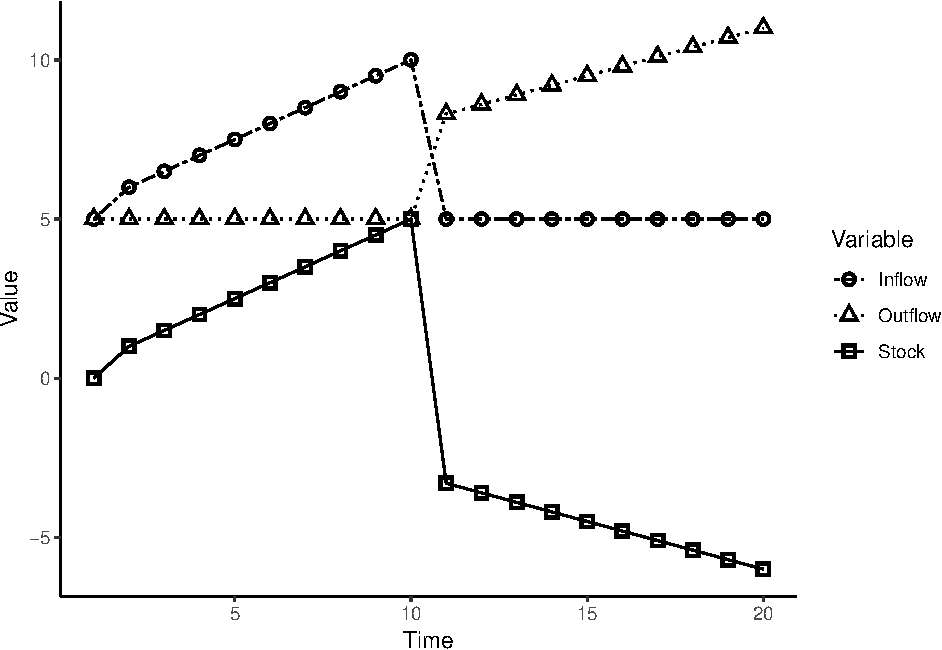
\includegraphics{compile_cp_files/figure-latex/unnamed-chunk-4-1.pdf}
\caption{\label{fig:unnamed-chunk-4}something\label{stocks}}
\end{figure}

\noindent Beginning at the first time point, inflows are equal to
outflows and the stock therefore sits at zero. Over the first ten time
points, however, outflows remain the same whereas inflows increase. With
inflows exceeding outflows the stock also increases up until time point
ten. At this time, inflows drop back down to five whereas outflows
increase -- leading to a large reduction in the stock. As outflows
continue to rise over time with no counterbalancing movement from the
inflow, the stock ultimately decreases.

Systems theory uses stocks and flows as general labels for each of the
things in the system. Above, we described the behavior of the stocks and
flows with simple terms -- increasing, decreasing, or constant. Systems
theory also provides a more systematic way of describing trajectories
and explaining behavior over time. These are unpacked in an excellent
paper by Monge (1990), and the framework includes trend, magnitude, rate
of change, and periodicity. Each of these is shown respectively in
figure \ref{monge}.

\begin{figure}
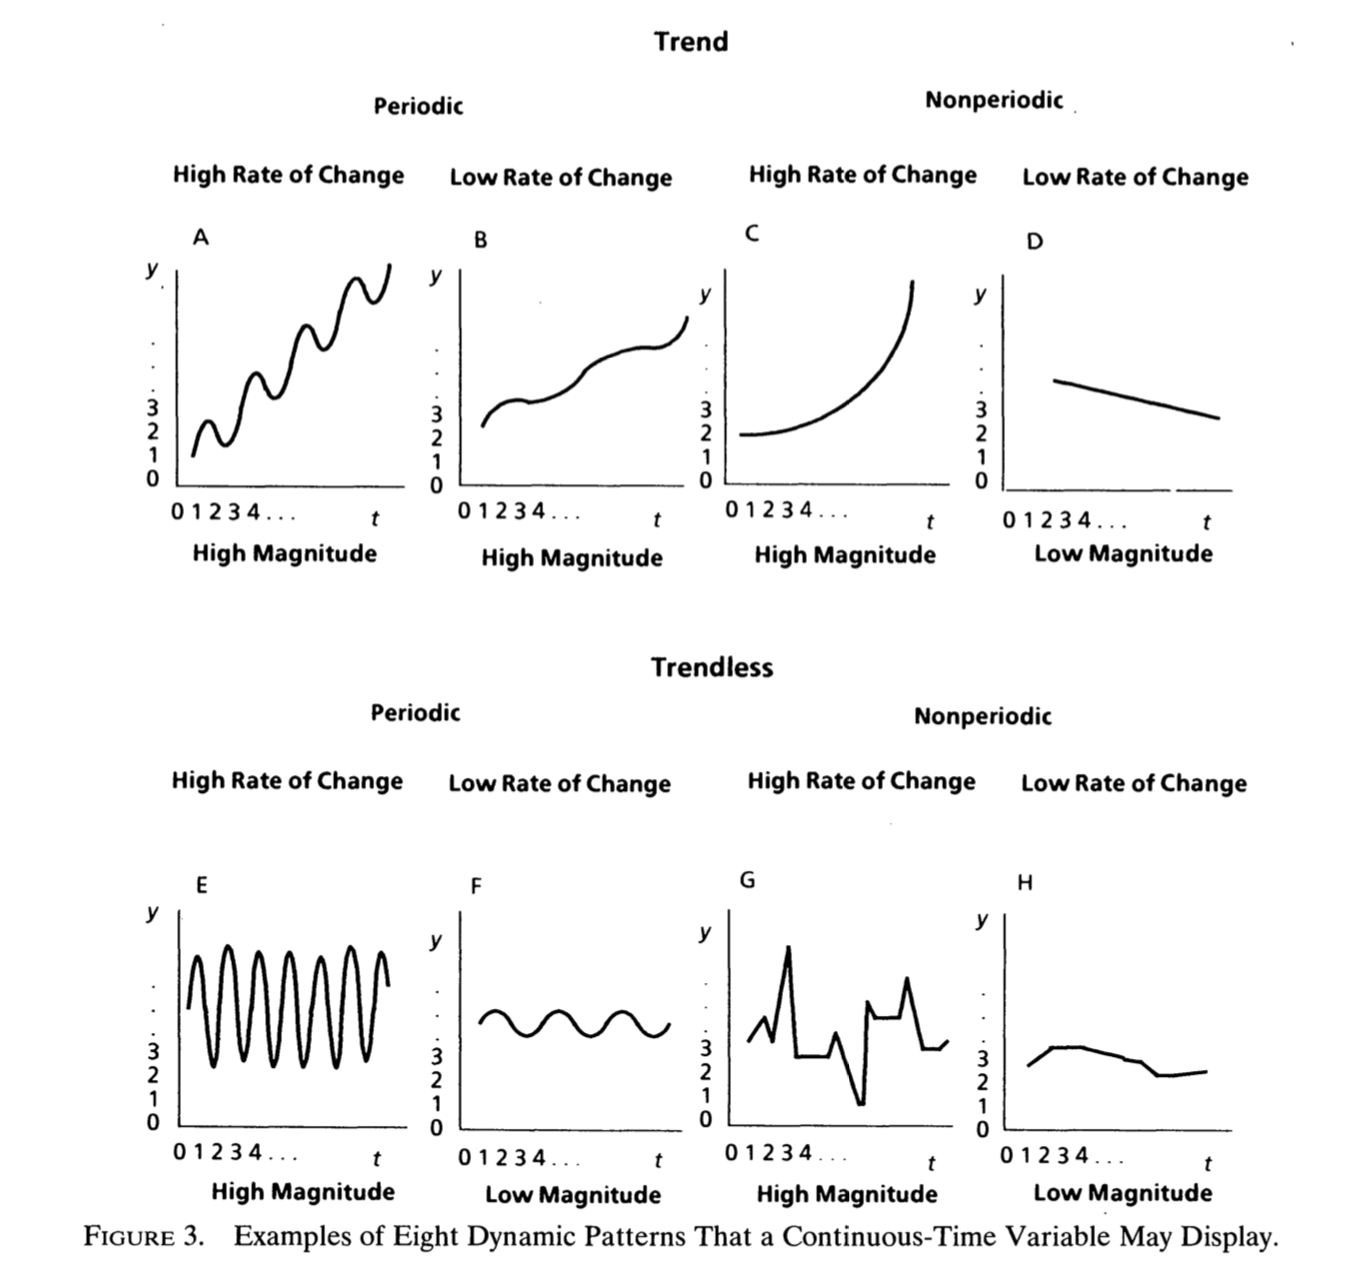
\includegraphics[width=3.42in]{figs/fig_monge1} \caption{something else\label{monge}}\label{fig:unnamed-chunk-5}
\end{figure}

\begin{center}

---------------

Insert Figure \ref{monge} Here

---------------

\end{center}

\hypertarget{trend}{%
\subsection{Trend}\label{trend}}

Dividing figure two into two portions -- the top and bottom -- reveals
differences in trend. All of the panels on the top of figure two have
trend, whereas those on the bottom do not. Trend is the systematic
increase or decrease of a variable over time.

\hypertarget{magnitude}{%
\subsection{Magnitude}\label{magnitude}}

Magnitude is the level, value, or amount of the variable at each time
point -- the number on the \(y\) axis at each respective point in time.
For example, in panel \emph{C} of figure two the magnitude is low at
times 1, 2, and 3, but is high at later points in time. Additionally,
panel \emph{E} and \emph{F} have the same magnitude if we average their
values over time, but panel \emph{E} contains both high and low
magnitude, whereas the magnitude for the trajectory in panel \emph{F}
remains relatively constant.

\hypertarget{rate-of-change}{%
\subsection{Rate of Change}\label{rate-of-change}}

Monge refers to rate of change as \enquote{How fast the magnitude
increases or decreases per one unit of time.} Panels \emph{G} and
\emph{H} reveal differences in rates of change.

\hypertarget{periodicity-cycles-oscillations}{%
\subsection{Periodicity; Cycles;
Oscillations}\label{periodicity-cycles-oscillations}}

Periodicity is the amount of time before a pattern repeats itself, and
it is equivalent to terms like cycles or oscillations. The most
important piece about periodicity is that it must be couched with
\enquote{controlling for trend.} Notice that panel \emph{A} is periodic
because, after controlling for trend, there are repeated patterns over
time.

\hypertarget{now-two-variables}{%
\subsection{Now two variables}\label{now-two-variables}}

It is of course possible to combine these notions when researchers are
studying processes with more than one variable. For example, a
researcher might describe the magnitude in their presumed dependent
variable with respect to the magnitude of their independent variable, or
the rates of change across the system of variables. When we turn to the
behavior and relationships among a system of variables a few additional
principles are available.

\hypertarget{lags}{%
\subsection{Lags}\label{lags}}

How long does it take for the presumed independent variable to produce
an effect on the outcome? This is the notion of lag.

\hypertarget{permanence}{%
\subsection{Permanence}\label{permanence}}

Once the effect happens, how long does it last?

\hypertarget{feedback-loops}{%
\subsection{Feedback Loops}\label{feedback-loops}}

Systems theory researchers often put feedback loops as a central
component to their discussion or analysis. This idea is also a common
explanation in our own literature. Feedback loops describe processes
where a variable eventually relates back to itself. For example, EXAMPLE
HERE.

Researchers often focus on the behavior that results as a function of
this feedback. When feedback causes the variable to move in the opposite
direction than it initially moved, this is known as negative feedback,
deviation counteraction, or a balancing feedback loop ({\textbf{???}};
{\textbf{???}}). Here, an initial increase in \(x\) leads to subsequent
changes in the system that, through time, eventually cause \(x\) to
decrease. Now that \(x\) has gone down, more changes happen in the
system that, through time, eventually cause \(x\) to increase.

When feedback, instead, causes the variable to move in the same
direction that it initially moved, this is known as postive feedback,
deviation ampliciation, or a reinforcing feedback loop ({\textbf{???}};
{\textbf{???}}). Here, changes in \(x\) in one direction lead to
eventual changes in \(x\) in the same direction and thus produce
exponential, explosive, or amplifying behavior.

\hypertarget{summary}{%
\subsection{Summary}\label{summary}}

These systems theory notions are valuable tools to explain and describe
process. Note that we did not cover everything to keep the reading
concise and consistent. For example, ({\textbf{???}}) also covers
discontinuous systems, so please refer to his excellent paper for an
even deeper discussion. Now we turn to mathematics and statistics and
describe principles from these domains that are used to explain process.

\hypertarget{mathematical-statistical-and-dynamics-principles}{%
\section{Mathematical, Statistical and Dynamics
Principles}\label{mathematical-statistical-and-dynamics-principles}}

\hypertarget{difference-equations}{%
\subsection{Difference Equations}\label{difference-equations}}

In mathematics, a basic representation of a process over time is a
difference equation:

\begin{equation}
\label{basicD}
y = y_{t - 1}
\end{equation}

\noindent where the value of \(y\) is the same at each \(t\), and the
emergent behavior would be a flat line across time. In systems theory
terms, there would be no trend.

Although equation \ref{basicD} seems simple, it introduces a fundamental
concept in dynamics: memory. The variable now depends on where it was in
the past. It is constrained, there are boundaries on where it can go.

As we add terms to this basic difference equation the behavior of the
variable becomes more complex. Adding a forcing constant, \emph{c} in
equation \ref{basicD} produces positive or negative trend depending on
whether \emph{c} is, respectively, positive or negative. For example,
the following equation:

\begin{equation}
\begin{split}
\label{diffC}
y &= y_{t-1} + c \\ 
c &= -4
\end{split}
\end{equation}

\noindent produces a line that decreases by four units at each time
point.

Autoregressive terms represent the extent to which the variable relates
to itself over time. Here:

\begin{equation}
\begin{split}
\label{diffA}
y &= a y_{t-1} \\ 
a &= 0.5
\end{split}
\end{equation}

\noindent the variable is described over time but it does not retain the
same value at each \(t\). Instead, the variable is \emph{similar} over
time and the autoregressive term, \(a\), describes the extent of that
similarity. The term is 0.5, meaning that the relationship between the
variable now and itself at the next time point will be 0.5.

There are fundamental properties of dynamic variables based on their
autoregressive terms, and these are shown in figure \ref{dynamics_plot}.
The top row of figure \ref{dynamics_plot} shows the trajectory of a
variable with autoregressive terms that are greater than one in absolute
value. These large terms produce explosive behavior -- exponential
growth when \(a\) is positive and oscillating CHAOS? when \(a\) is
negative. When the autoregressive term falls between zero and one,
conversely, the variable converges to an equilibrium value -- shown in
the bottom two panels. Either the variable oscillates at a decreasing
rate until it reaches equilibrium (when \(a\) is negative) or it
converges there smoothly (when \(a\) is positive).

\begin{figure}
\centering
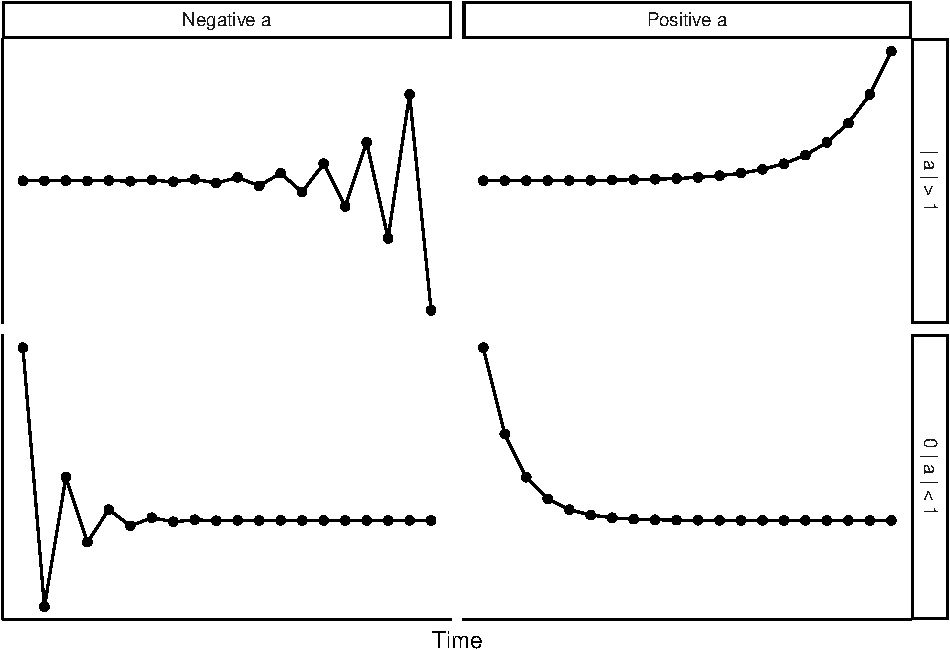
\includegraphics{compile_cp_files/figure-latex/unnamed-chunk-6-1.pdf}
\caption{\label{fig:unnamed-chunk-6}something here\label{dynamics_plot}}
\end{figure}

\begin{center}

---------------

Insert Figure \ref{dynamics_plot} Here

---------------

\end{center}

\hypertarget{stochastics}{%
\subsection{Stochastics}\label{stochastics}}

\hypertarget{random-walks}{%
\subsection{Random Walks}\label{random-walks}}

\hypertarget{stationarity}{%
\subsection{Stationarity}\label{stationarity}}

\hypertarget{cointegration}{%
\subsection{Cointegration}\label{cointegration}}

\hypertarget{granger-causality-and-directionality}{%
\subsection{Granger Causality and
Directionality}\label{granger-causality-and-directionality}}

X granger causes Y if Y can be better predicted by the histories of both
X and Y than the history of Y alone. If lagged values of X help predict
current values of Y in a forecast formed from lagged values of both X
and Y, then X is said to Granger cause Y. We implement this notion by
regressing eggs on lagged eggs and lagged chickens; if the coefficients
on lagged chickens are significant as a group, then chickens cause eggs.
A symetric regression tests the reverse causality. We perform the
Granger causality tests using one to four lags. The number of lags in
each equation is the same for eggs and chickens. To conclude that one of
the two \enquote{came first,} we must find unidirectional causality from
one to the other. In other words, we must reject the noncausality of the
one to the other and at the same time fail to reject the noncausality of
the other to the one. If either both cause each other or neigher causes
the other, the question will remain unanswered. Results reject that eggs
do not Granger cause chickens. They provide no such reject of the
hypothesis that chickens do not Granger cause eggs. Therefore, we
conclude that eggs cause chickens. A better phrasing might be
\enquote{temporally related} (Granger \& Newbold, p.~225) -- Thurman and
Fisher 1988 call it temporally ordered.

\hypertarget{diffusion}{%
\subsection{Diffusion}\label{diffusion}}

\hypertarget{damping}{%
\subsection{Damping}\label{damping}}

\hypertarget{markov-process}{%
\subsection{Markov Process}\label{markov-process}}

\newpage

\hypertarget{references}{%
\section{References}\label{references}}

\setlength{\parindent}{-0.5in}
\setlength{\leftskip}{0.5in}


\end{document}
